\documentclass[border=8pt]{standalone}
\usepackage[dvipsnames,svgnames]{xcolor}
\usepackage{amsmath}
\usepackage{amssymb}
\usepackage{tikz}
\usetikzlibrary{
  arrows.meta,
  positioning,
  calc,
  fit,
  backgrounds,
  decorations.pathreplacing,
  shapes.geometric,
  shadows.blur
}

\begin{document}
\begin{figure}[htbp]
\centering
\resizebox{\textwidth}{!}{%
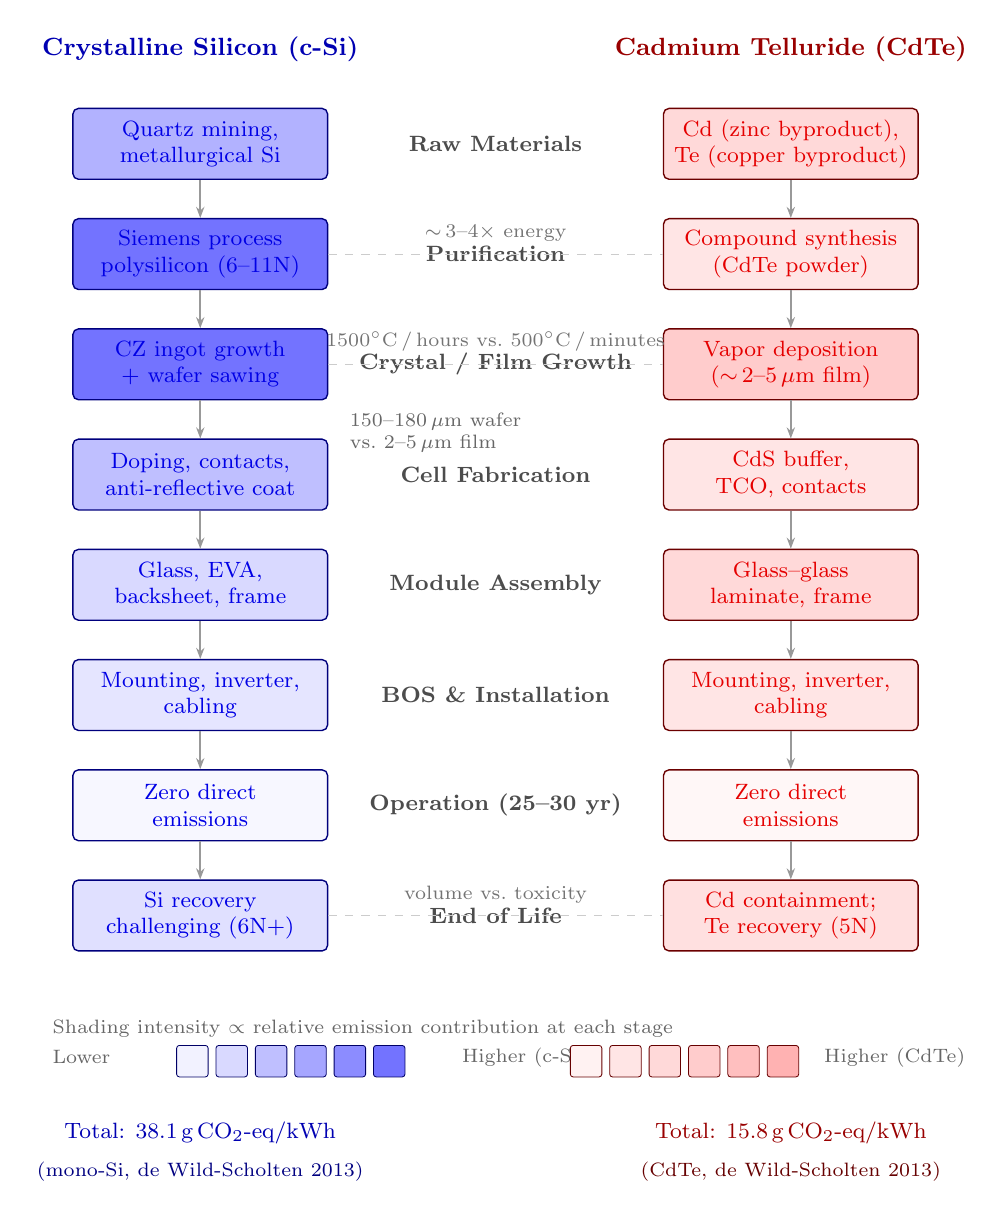
\begin{tikzpicture}[
    % Base styles
    >=Stealth,
    node distance=0.6cm and 2.0cm,
    % Box styles with parametric fill
    stage/.style={
        rectangle,
        rounded corners=2pt,
        draw=#1!70!black,
        line width=0.5pt,
        minimum height=0.9cm,
        text width=3.0cm,
        align=center,
        font=\footnotesize,
    },
    % c-Si stages: blue family, darker fill = higher emission share
    csi/.style={stage={blue!70!black}, fill=blue!#1, text=blue!90!black},
    % CdTe stages: red/coral family
    cdte/.style={stage={red!60!black}, fill=red!#1, text=red!90!black},
    % Shared/common stages: gray
    shared/.style={stage={gray!60!black}, fill=gray!#1, text=gray!90!black},
    % Label style
    stagelab/.style={
        font=\footnotesize\bfseries,
        text=black!70,
    },
    % Arrow style
    flow/.style={
        -{Stealth[length=4pt, width=3pt]},
        line width=0.6pt,
        color=black!40,
    },
    % Annotation style
    annot/.style={
        font=\scriptsize,
        text=black!60,
        align=left,
        text width=3.2cm,
    },
    % Column header
    colhead/.style={
        font=\small\bfseries,
        text=black!80,
    },
]
 
% ---------------------------------------------------------------
% Column headers
% ---------------------------------------------------------------
\node[colhead, text=blue!70!black] (hcsi) at (0, 0) {Crystalline Silicon (c-Si)};
\node[colhead, text=red!60!black]  (hcdte) at (7.5, 0) {Cadmium Telluride (CdTe)};
 
% ---------------------------------------------------------------
% Stage labels (center column)
% ---------------------------------------------------------------
\node[stagelab] (L1) at (3.75, -1.2) {Raw Materials};
\node[stagelab] (L2) at (3.75, -2.6) {Purification};
\node[stagelab] (L3) at (3.75, -4.0) {Crystal / Film Growth};
\node[stagelab] (L4) at (3.75, -5.4) {Cell Fabrication};
\node[stagelab] (L5) at (3.75, -6.8) {Module Assembly};
\node[stagelab] (L6) at (3.75, -8.2) {BOS \& Installation};
\node[stagelab] (L7) at (3.75, -9.6) {Operation (25--30 yr)};
\node[stagelab] (L8) at (3.75, -11.0) {End of Life};
 
% ---------------------------------------------------------------
% c-Si column (left) — fill intensity ~ emission share
%   Si purification and ingot growth are dominant stages
% ---------------------------------------------------------------
\node[csi=30] (S1a) at (0, -1.2) {Quartz mining,\\metallurgical Si};
\node[csi=55] (S2a) at (0, -2.6) {Siemens process\\polysilicon (6--11N)};
\node[csi=55] (S3a) at (0, -4.0) {CZ ingot growth\\+ wafer sawing};
\node[csi=25] (S4a) at (0, -5.4) {Doping, contacts,\\anti-reflective coat};
\node[csi=15] (S5a) at (0, -6.8) {Glass, EVA,\\backsheet, frame};
\node[csi=10] (S6a) at (0, -8.2) {Mounting, inverter,\\cabling};
\node[csi=3]  (S7a) at (0, -9.6) {Zero direct\\emissions};
\node[csi=12] (S8a) at (0, -11.0) {Si recovery\\challenging (6N+)};
 
% ---------------------------------------------------------------
% CdTe column (right) — much lower emission share at each stage
% ---------------------------------------------------------------
\node[cdte=15] (S1b) at (7.5, -1.2) {Cd (zinc byproduct),\\Te (copper byproduct)};
\node[cdte=10] (S2b) at (7.5, -2.6) {Compound synthesis\\(CdTe powder)};
\node[cdte=20] (S3b) at (7.5, -4.0) {Vapor deposition\\($\sim$\,2--5\,$\mu$m film)};
\node[cdte=10] (S4b) at (7.5, -5.4) {CdS buffer,\\TCO, contacts};
\node[cdte=15] (S5b) at (7.5, -6.8) {Glass--glass\\laminate, frame};
\node[cdte=10] (S6b) at (7.5, -8.2) {Mounting, inverter,\\cabling};
\node[cdte=3]  (S7b) at (7.5, -9.6) {Zero direct\\emissions};
\node[cdte=12] (S8b) at (7.5, -11.0) {Cd containment;\\Te recovery (5N)};
 
% ---------------------------------------------------------------
% Flow arrows — c-Si column
% ---------------------------------------------------------------
\draw[flow] (S1a.south) -- (S2a.north);
\draw[flow] (S2a.south) -- (S3a.north);
\draw[flow] (S3a.south) -- (S4a.north);
\draw[flow] (S4a.south) -- (S5a.north);
\draw[flow] (S5a.south) -- (S6a.north);
\draw[flow] (S6a.south) -- (S7a.north);
\draw[flow] (S7a.south) -- (S8a.north);
 
% ---------------------------------------------------------------
% Flow arrows — CdTe column
% ---------------------------------------------------------------
\draw[flow] (S1b.south) -- (S2b.north);
\draw[flow] (S2b.south) -- (S3b.north);
\draw[flow] (S3b.south) -- (S4b.north);
\draw[flow] (S4b.south) -- (S5b.north);
\draw[flow] (S5b.south) -- (S6b.north);
\draw[flow] (S6b.south) -- (S7b.north);
\draw[flow] (S7b.south) -- (S8b.north);
 
% ---------------------------------------------------------------
% Annotations — key differentiators at each stage
% ---------------------------------------------------------------
% Stage 2: Purification
\node[annot, anchor=west] at ($(L2.east)+(0.05,0)$) {};
\draw[dashed, gray!40, line width=0.4pt]
    (S2a.east) -- (S2b.west)
    node[midway, above=1pt, font=\scriptsize, text=black!55] 
    {$\sim$\,3--4$\times$ energy};
 
% Stage 3: Crystal/Film growth
\draw[dashed, gray!40, line width=0.4pt]
    (S3a.east) -- (S3b.west)
    node[midway, above=1pt, font=\scriptsize, text=black!55]
    {1500$^\circ$C\,/\,hours vs.\ 500$^\circ$C\,/\,minutes};
 
% Stage 3 annotation: wafer vs thin film
\node[annot, anchor=north west] at ($(S3a.south east)+(0.15,-0.03)$) {
    150--180\,$\mu$m wafer\\vs.\ 2--5\,$\mu$m film};
 
% Stage 8: End of life
\draw[dashed, gray!40, line width=0.4pt]
    (S8a.east) -- (S8b.west)
    node[midway, above=1pt, font=\scriptsize, text=black!55]
    {volume vs.\ toxicity};
 
% ---------------------------------------------------------------
% Emission intensity legend
% ---------------------------------------------------------------
\node[font=\scriptsize, text=black!60, anchor=north west] at (-2.0, -12.2) {
    Shading intensity $\propto$ relative emission contribution at each stage};
 
% Gradient legend boxes
\node[anchor=west, font=\scriptsize, text=black!60] at (-2.0, -12.8) {Lower};
\foreach \x/\f in {0/5, 0.5/15, 1.0/25, 1.5/35, 2.0/45, 2.5/55} {
    \fill[blue!\f, draw=blue!40!black, line width=0.3pt, rounded corners=1pt]
        (-0.3+\x, -13.05) rectangle (0.1+\x, -12.65);
}
\node[anchor=west, font=\scriptsize, text=black!60] at (3.2, -12.8) {Higher (c-Si)};
 
\foreach \x/\f in {5.0/5, 5.5/10, 6.0/15, 6.5/20, 7.0/25, 7.5/30} {
    \fill[red!\f, draw=red!40!black, line width=0.3pt, rounded corners=1pt]
        (-0.3+\x, -13.05) rectangle (0.1+\x, -12.65);
}
\node[anchor=west, font=\scriptsize, text=black!60] at (7.8, -12.8) {Higher (CdTe)};
 
% ---------------------------------------------------------------
% Summary totals at bottom
% ---------------------------------------------------------------
\node[font=\footnotesize, text=blue!70!black, anchor=north] at (0, -13.5) {
    Total: 38.1\,g\,CO$_2$-eq/kWh};
\node[font=\scriptsize, text=blue!50!black, anchor=north] at (0, -14.0) {
    (mono-Si, de Wild-Scholten 2013)};
 
\node[font=\footnotesize, text=red!60!black, anchor=north] at (7.5, -13.5) {
    Total: 15.8\,g\,CO$_2$-eq/kWh};
\node[font=\scriptsize, text=red!40!black, anchor=north] at (7.5, -14.0) {
    (CdTe, de Wild-Scholten 2013)};
 
\end{tikzpicture}
}% end resizebox
\label{fig:lifecycle_flowchart}
\end{figure}
\end{document}
